\documentclass[a4paper]{article}

\usepackage{amsmath}
\usepackage{amssymb}
\usepackage{parskip}    % skip line
\usepackage[backend=bibtex]{biblatex}   % references
\usepackage[hang]{subfigure}
\usepackage[noend]{algpseudocode}
\usepackage{algorithm}
\usepackage{makecell}
\usepackage{fvextra}
\usepackage{adjustbox}

\usepackage{lpi}

\addbibresource{./references.bib}
\graphicspath{ {./media} } % sections/images

\title{%
    Trimap Matting \\
    \phantom{} \\
    \large Scuola d'Arti e Mestieri di Trevano (SAMT) \\
    \large Documentation
}

\author{Paolo Bettelini}

\date{}

\lpisetup%
    {Trimap Matting}

\makenoidxglossaries

\newglossaryentry{FFI}
{
    name=FFI,
    description={Foreign Function Interface}
}

\newglossaryentry{trait}
{
    name=trait,
    description={A trait in Rust defined shared behavior among structures}
}

\begin{document}

\maketitle

\pagebreak

\tableofcontents

\pagebreak

\section{Introduction}

\subsection{Abstract}

Background removal has been a longstanding practice in digital image processing.
While removing the background from images with simple borders is relatively straightforward,
more complex borders, such as hair, require the use of more sophisticated techniques.
Trimap matting is a novel and effective approach to solving the latter.
This project involves the development of a user-friendly command-line and web graphical user interface
to make use of this algorithm.

\subsection{Information}

This is a project of the Scuola Arti e Mestieri di Trevano (SAMT) under the following circumstances

\begin{itemize}
    \item \textbf{Section}: Computer Science
    \item \textbf{Year:} Fourth
    \item \textbf{Class:} Progetti Individuali
    \item \textbf{Supervisor:} Geo Petrini
    \item \textbf{Title:} Trimap Matting
    \item \textbf{Start date}: 2022-12-12
    \item \textbf{Deadline}: 2023-04-06
\end{itemize}

and the following requirements

\begin{itemize}
    \item \textbf{Documentation}: a full documentation of the work done
    \item \textbf{Diary}: constant changelog for each working session
    \item \textbf{Source code}: source code of the project
\end{itemize}

All the source code and documents can be found at
\href{https://github.com/paolobettelini/trimap-matting}
{https://github.com/paolobettelini/trimap-matting}
\cite{gitrepo}.

\pagebreak

\section{Requirements}

\requirement{00}{CLI tool}{1}{1.1}{none}{
    A CLI tool to execute background removal must be developed.
}{
    \subreq{00}{0}{The target image must be specified.}
    \subreq{00}{1}{The trimap image can be specified.}
    \subreq{00}{2}{The soft mask can be specified.}
    \subreq{00}{3}{Either the soft mask or the trimap must be specified.}
    \subreq{00}{4}{The program can save the generated background mask.}
    \subreq{00}{5}{The program can remove the background and replace it with an image.}
    \subreq{00}{6}{The program can remove the background and fill it with a color.}
    \subreq{00}{7}{The program can remove the background and leave it transparent.}
}

\requirement{01}{Image formats}{1}{1.0}{none}{
    Multiple image formats must be supported.
}{
    \subreq{00}{0}{The JPG format must be supported.}
    \subreq{00}{1}{The PNG format must be supported.}
    \subreq{00}{2}{The WebP format must be supported.}
}

\requirement{02}{Size check}{1}{1.0}{none}{
    The executable must assert that the target image and trimap are of the same size.
}{%
}

\requirement{03}{GUI}{1}{1.0}{none}{
    A GUI application must be developed in other to interact with the program features.
}{%
}

\requirement{04}{Default name}{1}{1.0}{The name must be generated using the current timestamp.}{
    The mask and output files must be assigned a default name
    none is specified.
}{%
}

\requirement{05}{Logging}{1}{1.0}{none}{
    The programs must have logging capabilities
}{%
}

\pagebreak

\section{Trimap Matting}
\label{sec:trimat}

Matting is a technique used to extract an object
from an image.
Trimap matting is a term used to refer to the process
of generating alpha mattes\cite{matte} for an object
% https://en.wikipedia.org/wiki/Matte_(filmmaking)
in an image given an initial
approximation of its borders.

The goal of this process is to determine
how much each pixel of a target image is part of the
object that needs to be extracted.
This means that given a pixel \(P_{x,y}\)
we want to find a value \(\alpha \in \mathbb{R}\) such that
\[
    P_{x,y} = \alpha F_{x,y} + (1-\alpha) B_{x,y},
    \quad \alpha \in [0;1]
\]
where \(F\) represents the foreground color
and \(B\) represents the background color at a given pixel.

Note that the multiplicative operator here is the scalar vector multiplication.
This is because the pixels are represented by a vector of values,
usually \({\mathbb{R}}^3\) or \({\mathbb{R}}^4\) (for transparent images).

The trimap is an approximation of the alpha mattes.
The black dye represents background-only space, the white dye
represents foreground-only space whilst the gray one
delimits the distinction between the two.

Here are some examples using an image of a plant.

\begin{figure}[h]
    \begin{minipage}{0.33\textwidth}
        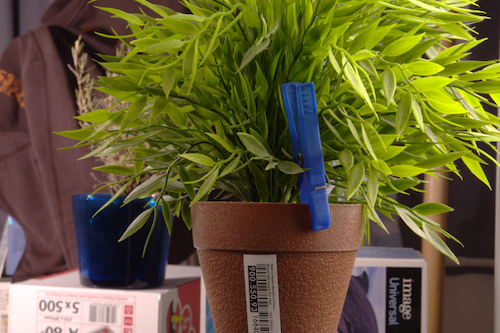
\includegraphics[width=\textwidth]{target.jpg}
        \caption{Plant Image}
    \end{minipage}
    \begin{minipage}{0.33\textwidth}
        
\includegraphics[width=\textwidth]{trimap.png}
        \caption{Plant Trimap}
    \end{minipage}
    \begin{minipage}{0.33\textwidth}
        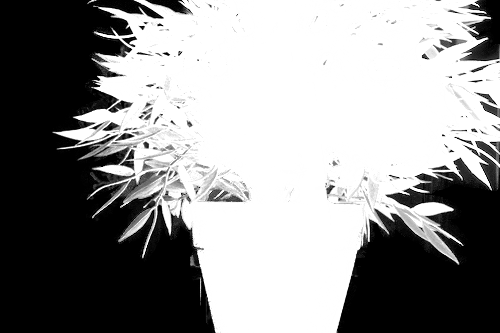
\includegraphics[width=\textwidth]{mask.png}
        \caption{Plant Soft Mask}
    \end{minipage}
\end{figure}

Once the alpha mattes are generated (soft mask) we can use them
to extract the object from the target image.
Thus, we can remove the background behind the object,
fill the background with a color, replace it with another image,
or leave it transparent.

Given a target image with pixels \(T_{x,y}\), the alpha
mattes \(\alpha_{x,y}\) and the pixels of the replacement image
\(R_{x,y}\) we can compute the pixels of the output image \(T_{x,y}'\)
as follows
\[
    T_{x,y}' = 
    \alpha_{x,y} \cdot T_{x,y} + (1 - \alpha_{x,y}) \cdot R_{x,y}
\]
If we want to replace the background with a color, we can consider.
\(R={(r,g,b)}^t\) \\
If we just want to leave the background transparent, meaning
\(T' \in {\mathbb{R}}^4\), we have
\[
    T_{x,y}' = 
    \alpha_{x,y} \cdot T_{x,y}
\]
and the alpha value for \(T_{x,y}\) is set to \(\alpha_{x,y}\).

\begin{figure}[h]
    \begin{minipage}{0.33\textwidth}
        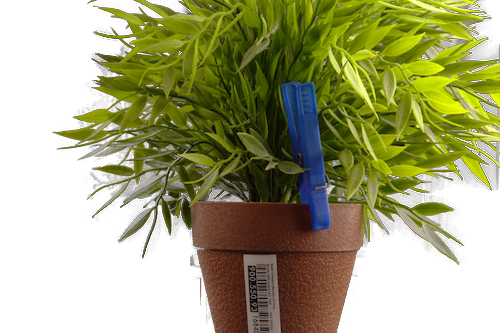
\includegraphics[width=\textwidth]{results/result3.png}
        \caption{Transparency}
    \end{minipage}
    \begin{minipage}{0.33\textwidth}
        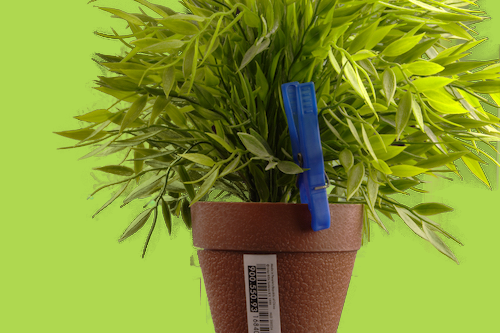
\includegraphics[width=\textwidth]{results/result2.png}
        \caption{Color fill}
    \end{minipage}
    \begin{minipage}{0.33\textwidth}
        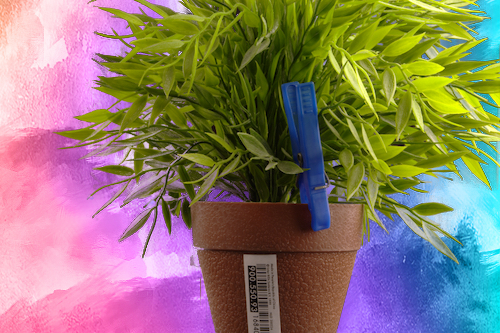
\includegraphics[width=\textwidth]{results/result1.png}
        \caption{Replacement}
    \end{minipage}
\end{figure}

\pagebreak

\section{Technologies}

\subsection{OpenCV}

\begin{wrapfigure}{r}{4cm}
    
\includegraphics[width=4cm]{opencvlogo.png}
\end{wrapfigure}

OpenCV\cite{opencv} is a library
for computer vision. It contains a large
amount of tools, from GUIs, video analysis, machine learning,
object detection, image processing and many more\cite{opencvdoc}.
The library also contains a module about \textit{alpha matting},
which contains a function to generate alpha mattes given a trimap
\cite{opencvalphamatting}.

\subsubsection{Trimap colors}

As stated in the last section, the gray color represents the unknown pixels.
The library, however, accepts a greyscale trimap.
The question is whether different grays have different meanings.
This is not documented and would require to read the original
paper of implementation. \\ % cite
In order to find out, here are a bunch of samples with different gray
colors:

\wrapfill

\begin{figure*}[h]
\makebox[\linewidth][c]{%
\centering
\subfigure[Trimap 1]{%
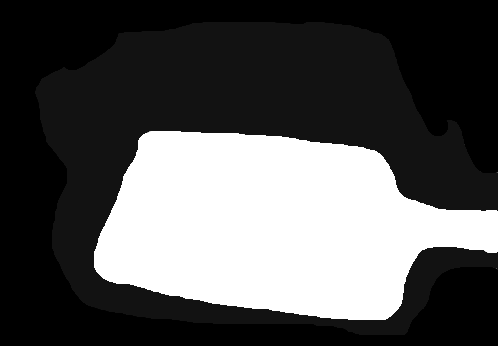
\includegraphics[width=0.25\textwidth]{brushes/trimap1.png}}%
\subfigure[Trimap 2]{%
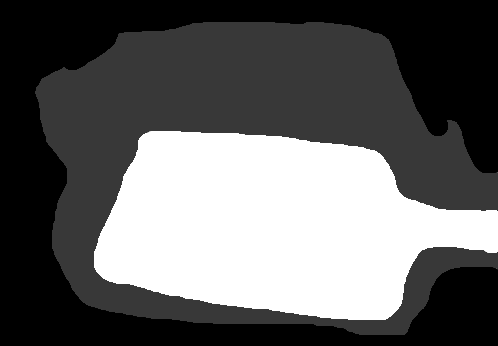
\includegraphics[width=0.25\textwidth]{brushes/trimap2.png}}%
\subfigure[Trimap 3]{%
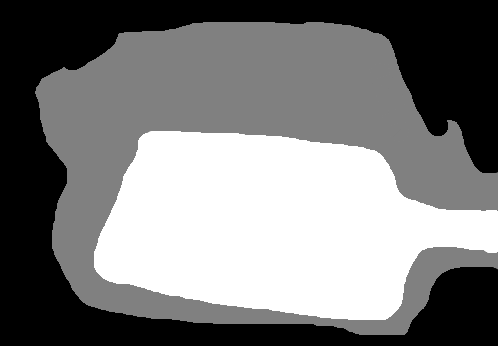
\includegraphics[width=0.25\textwidth]{brushes/trimap3.png}}%
\subfigure[Trimap 4]{%
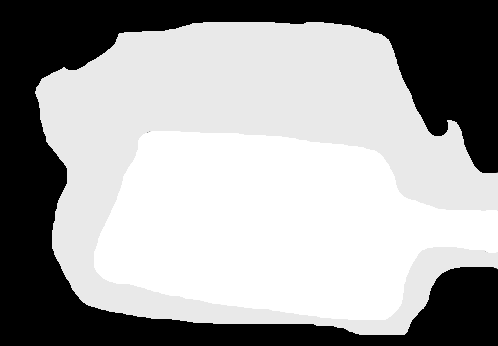
\includegraphics[width=0.25\textwidth]{brushes/trimap4.png}}%
}
\caption{Hairy brush trimaps}
\end{figure*}

\begin{figure*}[h]
\makebox[\linewidth][c]{%
\centering
\subfigure[Mask 1]{\label{fig:mask1}%
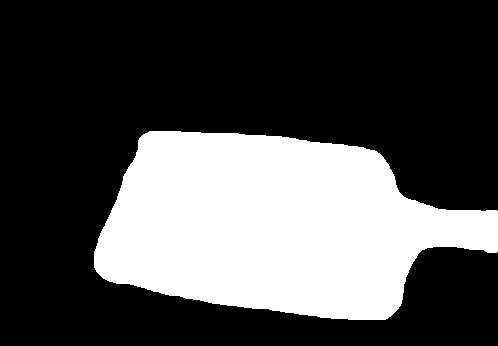
\includegraphics[width=0.25\textwidth]{brushes/mask1.png}}%
\subfigure[Mask 2]{\label{fig:mask2}%
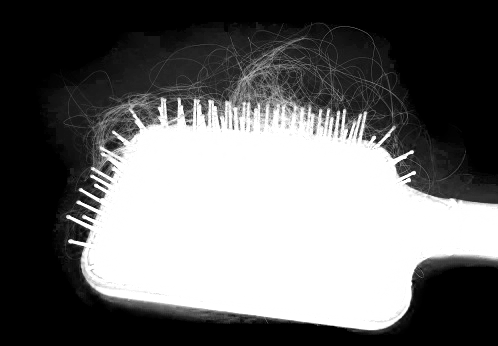
\includegraphics[width=0.25\textwidth]{brushes/mask2.png}}%
\subfigure[Mask 3]{\label{fig:mask3}%
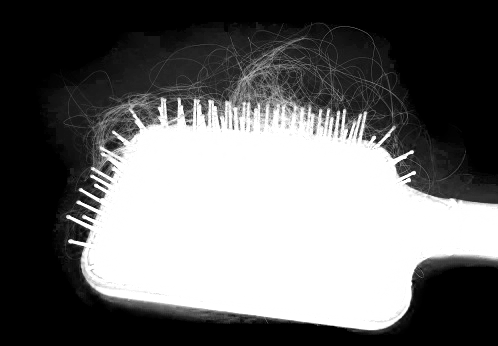
\includegraphics[width=0.25\textwidth]{brushes/mask3.png}}%
\subfigure[Mask 4]{\label{fig:mask4}%

\includegraphics[width=0.25\textwidth]{brushes/mask4.png}}%
}
\caption{Hairy brush masks}
\end{figure*}
%
\begin{wrapfigure}{l}{7cm}
    \vspace{-\intextsep}
    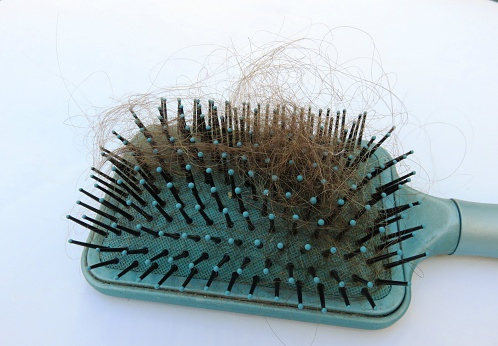
\includegraphics[width=7cm]{brushes/brush.jpg}
    \caption{Hairy brush}
\end{wrapfigure}

Given that this is the original image, we can confidently
infer that different gray values have the same meaning.
However, there is a range according to which a color is considered
\texttt{black}, \texttt{gray} or \texttt{white}.
As we can see in \ref{fig:mask1} and \ref{fig:mask4},
the unknown pixels have been considered to be background
or foreground respectively, because the gray value was too
low or too high.

\wrapfill

\pagebreak

\subsection{Rust}

Rust\cite{rust} is a generic compiled programming language.
The code is compiled using LLVM to machine code and its speed
is comparable to C and C++.
Rust is the first programming language to guarantee memory safety;
memory is not manually freed nor garbage collected.
It is not possible to dereference a null pointer, cause memory segfaults, core dumps
and memory leaks.
Code that could cause undefined behavior can still be written,
but it is strictly bounded in blocks where the compiler is relaxed.
This relaxation implies that the language is also low-level.
Another key feature to the performance of Rust is zero cost abstraction,
which means that generic types and function abstractions are resolved at compile-time.
Conditional compilation and compile-time computations are also extensively used.
\\
There are also many features concerning the programming experience, such as
advanced metaprogramming and code generation using macros, intelligent compiler,
dependency system (Cargo), modern syntax and many tools to ease development.

\textbf{\color{red} Note}: a Rust \textit{crate} refers to a library.
A \textit{feature} is an optional component of library.
A \textit{module} is a logical section of a program or library.

\pagebreak

\section{Compilation and usage}

\subsection{CLI}

\subsubsection{Compilation}

The executable can be compiled using the \texttt{cargo}
package manager.

\begin{lstlisting}[style=boxed]
    $ cd matting-cli
    $ cargo build --release
\end{lstlisting}

This will generate an executable (\texttt{matting-cli})
in \texttt{./target/release}.
In order to make this executable globally available,
you can move it into a folder in the \textsc{\$PATH} environment
variable, such as \texttt{/usr/bin}.
Ye may also modify the executable file name to change its invocation
name.

\begin{lstlisting}[style=boxed]
    $ sudo mv target/release/matting-cli /usr/bin/
\end{lstlisting}

The executable can now be invoked by just writing
\begin{lstlisting}[style=boxed]
    $ matting-cli
\end{lstlisting}

\subsubsection{Usage}

The following shows the output of the command upon
setting the \texttt{--help} or \texttt{-h} flag.
\begin{lstlisting}[style=boxed]
Matting CLI

Usage: matting-cli [OPTIONS] --target <TARGET>
                   <--mask <MASK>|--trimap <TRIMAP>>

Options:
  -i, --target <TARGET>        Target image
      --mask <MASK>            Background mask image
      --trimap <TRIMAP>        Trimap image
      --save-mask <SAVE_MASK>  Save mask path
  -o, --output <OUTPUT>        Output image
  -f, --fill <FILL>            Fill background action
  -t, --transparent            Transparent background action
  -r, --replace <REPLACE>      Replace background action
      --verbose                Verbose flag
  -h, --help                   Print help information
  -V, --version                Print version information
\end{lstlisting}

The \texttt{--target} parameter specifies the image
on which the operation needs to be applied.
This parameter is \underline{mandatory}.

The \texttt{--trimap} parameter specifies the trimap
image which will be used to generate the alpha mattes.

The \texttt{--mask} parameter specifies the image
containing the alpha mattes to use.

The parameter \texttt{--trimap} and \texttt{--mask}
are mutually exclusive, and one of them is \underline{mandatory}.

The advantage of using \texttt{--mask} over
\texttt{--trimap} is that the alpha mattes are
already given rather than having to be computed.
This can save lots of computational times.
The alpha mattes image can be saved on the file system
by specifying the \texttt{--save-mask} parameter.

The parameter \texttt{--save-mask} can either specify a filename
for the mask. If left blank, the program will generate a name (PNG format)
using the timestamp.

There are 3 different operations that can be applied
to the background of the result: \texttt{--transparent},
\texttt{--replace} or \texttt{--fill}.
These operations are mutually exclusive, and if one is specified,
the \texttt{--output} parameter can be set to
specify the path where the resulting image will be saved.
If the \texttt{--output} parameter is not specified then it will produce
a file name with the current timestamp.

\textbf{Note:} the argument of \texttt{--color} can be any valid
CSS color. See \cite{csscolors} for the documentation.

The \texttt{--verbose} flag is optional and will print additional
information about what the program is doing and the elapsed
time of each operation. Se the logging section for more information.

\subsubsection{Examples}

The following command generates a mask of the alpha mattes
given a trimap and saves it to \texttt{mask.png}.
\begin{lstlisting}[style=boxed]
    $ matting-cli -i target.jpg --trimap trimap.png
        --save-mask mask.png
\end{lstlisting}

The following command generates a mask of the alpha mattes
given a trimap and saves it to a file (e.g. \texttt{mask\_20230313-133117.png}).
\begin{lstlisting}[style=boxed]
    $ matting-cli -i target.jpg --trimap trimap.png
        --save-mask
\end{lstlisting}

The following command removes the background of an image
given its mask.
\begin{lstlisting}[style=boxed]
    $ matting-cli -i target.jpg --mask mask.png
        -o out.png --transparent
\end{lstlisting}

The following command removes the background of an image
given its mask and replaces it with the color \texttt{\#A3BF13}.
\begin{lstlisting}[style=boxed]
    $ matting-cli -i target.jpg --mask mask.png
        -o out.png --fill "#A3BF13"
\end{lstlisting}

The following command removes the background of an image
given its mask and replaces it with the image \texttt{background.png}.
\begin{lstlisting}[style=boxed]
    $ matting-cli -i target.jpg --mask mask.png
        -o out.png --replace background.png
\end{lstlisting}

The following command removes the background of an image
given its mask and leaves it transparent. The output is saved to a file
(e.g. \texttt{target\_20230313-134153.png}).
\begin{lstlisting}[style=boxed]
    $ matting-cli -i target.jpg --mask mask.png
        --transparent
\end{lstlisting}

The following shows the output of the program when the \texttt{--verbose}
flag is set. This command computes the alpha mattes given a trimap,
then it saves the generated mask, fills the background of the image
with the color red, and then saves the result.
\begin{lstlisting}[style=boxed]
    $ matting-cli -i target.jpg --trimap trimap.png
        --save-mask mask.png -o out.png --fill red --verbose
    
    Reading target image... Done! [4.021485ms]
    Reading trimap image... Done! [1.976477ms]
    Generating soft mask... Done! [7.104532642s]
    Reading target image... Done! [178.884124ms]
    Saving soft mask... Done! [509.050896ms]
    Filling background with color... Done! [117.90393ms]
    Saving output... Done! [954.085622ms]
\end{lstlisting}

\pagebreak

\subsection{Web application}

\subsubsection{Compilation}

The executable can be compiled using the \texttt{cargo}
package manager.

\begin{lstlisting}[style=boxed]
    $ cd matting-web
    $ cargo build --release
\end{lstlisting}

This will generate an executable (\texttt{matting-web})
in \texttt{./target/release}.
In order to make this executable globally available,
you can move it into a folder in the \textsc{\$PATH} environment
variable, such as \texttt{/usr/bin}.
You may also modify the executable file name to change its invocation
name.

\begin{lstlisting}[style=boxed]
    $ sudo mv target/release/matting-web /usr/bin/
\end{lstlisting}

The executable can now be invoked by just writing
\begin{lstlisting}[style=boxed]
    $ matting-web
\end{lstlisting}

\subsubsection{Usage}

The following shows the output of the command upon
setting the \texttt{--help} or \texttt{-h} flag.
\begin{lstlisting}[style=boxed]
Matting WEB

Usage: matting-web [OPTIONS] --www <WWW>

Options:
    -w, --www <WWW>            WWW static files folder
    -a, --address <ADDRESS>    Listening address [default: 0.0.0.0]
    -p, --port <PORT>          Listening port [default: 8080]
    -l, --log-file <LOG_FILE>  Log file
    -h, --help                 Print help
    -V, --version              Print version
\end{lstlisting}

The \texttt{--www} parameter specifies the path
of the static website files.
This parameter is \underline{mandatory}.

The \texttt{--address} parameter specifies the listening
address of the server.

The \texttt{--port} parameter specifies the listening
port of the server.

The \texttt{--log-file} parameter specifies a file to log to instead of the
\textsc{STDOUT} and \textsc{STDERR}.

\subsubsection{Examples}

The following command starts the server using the default
address and port (\texttt{0.0.0.0:8080}).
\begin{lstlisting}[style=boxed]
    $ matting-web --www /path/to/wwww
\end{lstlisting}

The following command starts the server listening to
(\texttt{::1:80}).
\begin{lstlisting}[style=boxed]
    $ matting-web -w /path/to/wwww -a ::1 -p 80
\end{lstlisting}

The following command starts the server and logs everything to a file.
\begin{lstlisting}[style=boxed]
    $ matting-web -w /path/to/wwww -l logfile.log
\end{lstlisting}

% Ancient length stuff
\newlength{\mtL}

% for A4
\setlength{\mtL}{.8\paperheight}% the next hsize
% FOR A3
%\setlength{\mtL}{1.4\paperheight}

\addtolength\mtL{-\headwidth}
\newpage
\addtolength\headwidth{\mtL}

% Flip Page

% for A3
%\pdfpagewidth=2\paperwidth
% FOR A4
\pdfpageheight=\paperwidth
\pdfpagewidth=\paperheight
\paperwidth=\pdfpagewidth
\paperheight=\pdfpageheight

% Text width and height
\begingroup
\vsize=1.125\pdfpageheight % set whatever you like
\hsize=1.125\pdfpageheight
\textwidth=\hsize
\textwidth=\vsize

% -- CONTENT --

\section{Planning}

\subsection{Initial Gantt Chart}

\begin{figure}[h]
    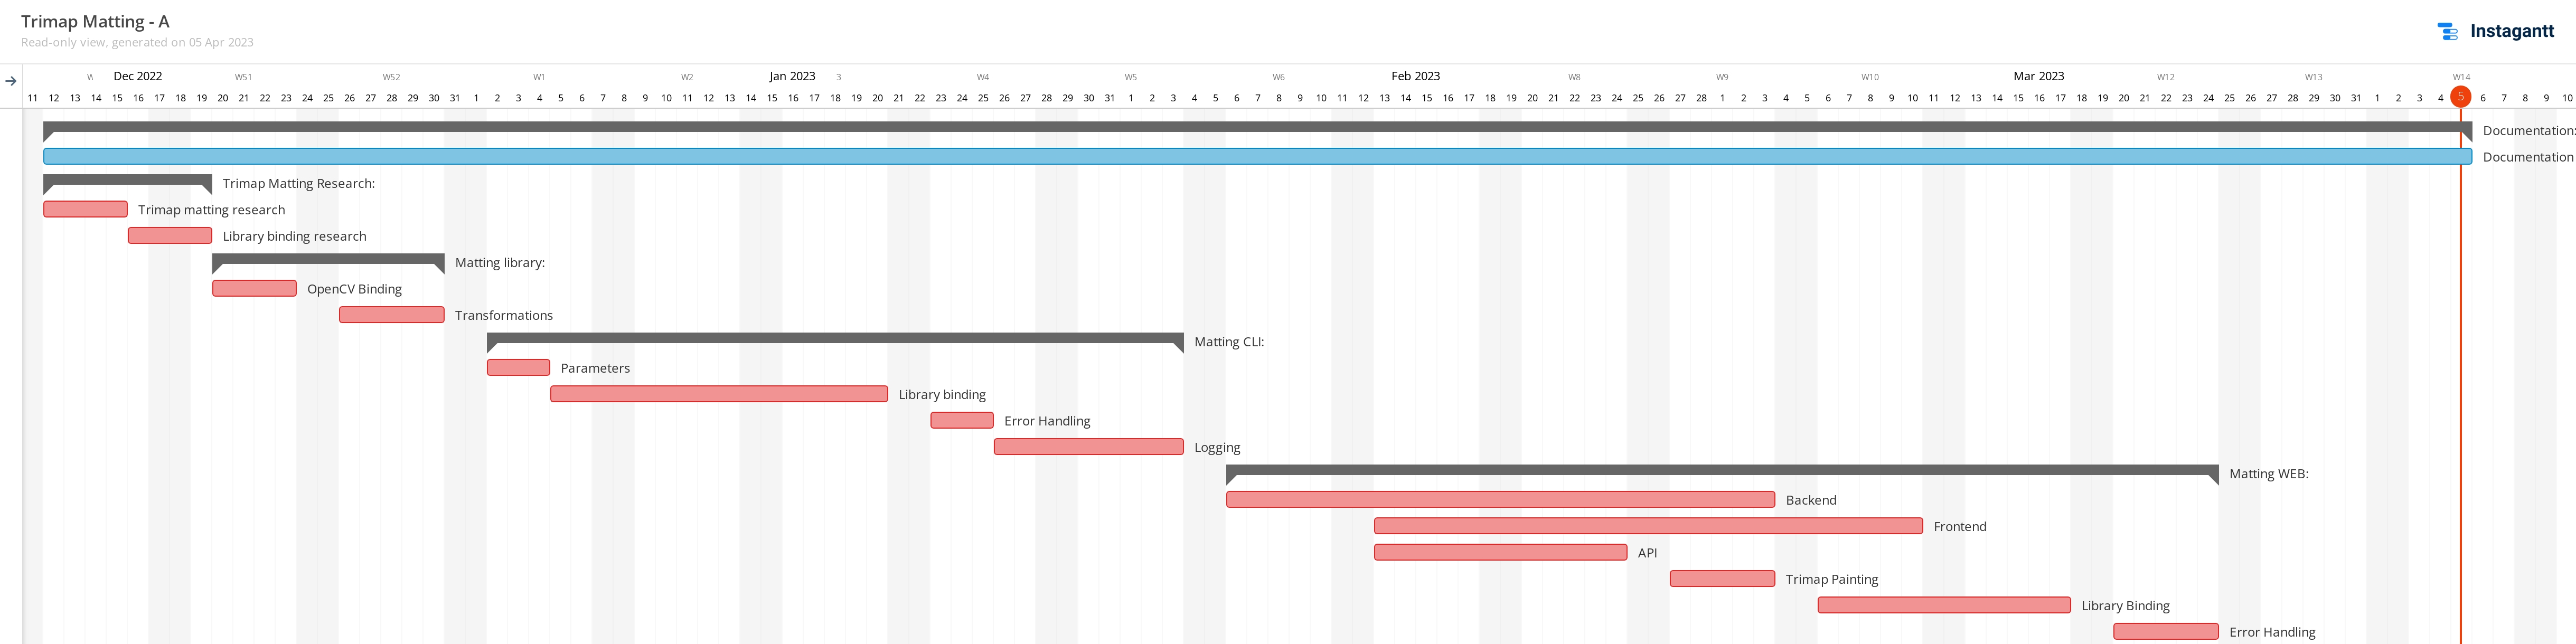
\includegraphics[width=\textwidth]{gantt/gantt1.jpg}
    \caption{Initial Gantt Chart}
\end{figure}

\newpage

\subsection{Final Gantt Chart}

% -- CONTENT --

\endgroup
\newpage
\addtolength\headwidth{-1\mtL}

% Unflip page

% FOR A3
%\pdfpagewidth=\paperwidth
% FOR A4
\paperwidth=\pdfpageheight
\paperheight=\pdfpagewidth
\pdfpageheight=\paperheight
\pdfpagewidth=\paperwidth

\section{Implementation}

\subsection{OpenCV fundamental types}

The fundamental OpenCV type used in this project is the
\textbf{Mat}\cite{mat} type. A mat is essentially an
\(n\)-dimensional array. It can represent tensors, vector fields,
matrices and much more, both with real numbers or complex numbers.
For the purpose of this project, any mat represents a grayscale
or a colored image.

\subsection{OpenCV Binding}

The OpenCV library is primarily written in C++.
In order to access its functions in Rust, I used a crate
called \texttt{opencv}\cite{rustopencv}, which is a binding
to the \gls{FFI} of opencv.

It does not fully implement the Rust idioms and best practices,
I found it very easy to accidentally cause a core dump
whilst calling a function.

The \textit{Flow Alpha Matting} module was developed by Muskaan Kularia
at Google Summer of Code 2019.

The code of interest is in the \texttt{opencv::alphamat} module,
and it contains the following function which computes alpha mattes of an object in an image.

\begin{lstlisting}[style=Rust, style=boxed]
    pub fn into_flow(
        image: &dyn ToInputArray,
        tmap: &dyn ToInputArray,
        result: &dyn ToOutputArray,
    ) -> Result<()>
\end{lstlisting}

\paragraph{Parameters:}
\begin{itemize}
    \item \textbf{image:} Input RGB image
    \item \textbf{tmap:} Input greyscale trimap image
    \item \textbf{result:} Output alpha matte image
\end{itemize}

The function intoFlow performs alpha matting on a RGB image
using a greyscale trimap image, and outputs a greyscale alpha matte image. \\
The output alpha matte can be used to softly extract the foreground
object from a background image. % cite

The \gls{trait}s \texttt{ToInputArray} and \texttt{ToOutputArray}
are implemented by the \texttt{Mat} type.

\pagebreak

\subsection{Core dump handling}

The opencv matting module will crash if the parameters
are incorrect. For instance, the image parameters are represents by a
\texttt{Mat} structure, and if the mats are of different sizes or have different color depth,
the library may try to access a mat as if it was bigger, causing a memory segmentation
and a core dump.

These incidents can be prevented by checking the size of the image and ensuring the correct
color depth before calling the library, however, some incidents are harder
to predict; if the trimap is only white (foreground) or only black (background),
then the library will cause a core dump. \\
It is also possible to prevent these crashes by checking every single pixel
of the canvas, however, I decided not do so because it is practically impossible
to prevent every (obscure) core dump. There may be more strange core dumps
that I have not encountered.

In order to fix this issue and prevent the server from abruptly stopping,
the trimap matting operations are implemented by calling the \texttt{matting-cli}
tool. This will start a secondary process. If the secondary process crashes,
the server mustn't be impacted. The images are passed to the other software using
temporary file in the \texttt{/tmp} directory (automatic cleanup
is ensured by the Rust memory safety model).

Although it works, this solution is not how I would have wished to have implemented
the functionality. For this reason, I also implemented the direct FFI call. \\
By compiling with the feature \textit{no\_matting\_cli}, e.g.
\begin{lstlisting}[style=Rust, style=boxed]
    cargo build --release --features no_matting_cli
\end{lstlisting}
the program will not call the \texttt{matting-cli} executable.

\pagebreak

\subsection{API Routes}

The routes are the following.
Note that each of them must include
a \texttt{multipart/form-data} attribute.

\begin{itemize}
    \item \textbf{POST}: \textbf{/api/matting} \\
        This endpoint returns in image representing the alpha mattes mask. \\
        The caller must specify two images: \textbf{target} and \textbf{trimap}.
    \item \textbf{POST}: \textbf{/api/fill/<color>} \\
        This endpoint replaces the background with a given color. \\
        The caller must specify two images: \textbf{target} and \textbf{mask}.
    \item \textbf{POST}: \textbf{/api/transparent} \\
        This endpoint removes the background and leaves it transparent. \\
        The caller must specify two images: \textbf{target} and \textbf{mask}.
    \item \textbf{POST}: \textbf{/api/replace} \\
        This endpoint replaces the background with a given image. \\
        The caller must specify three images: \textbf{target}, \textbf{mask} and \textbf{replacement}.
\end{itemize}

\subsection{Matting library}

The core of this project is certainly the alpha matting algorithm.
In order to develop both a CLI and a GUI tool to
use this algorithm, I created a separate library (\texttt{matting-lib})
containing all the matting and image processing related functions.

The library exports the following functions, modules and structures

\begin{lstlisting}[style=Rust, style=boxed]
pub use image::{ImageFormat, DynamicImage};
pub use opencv::imgcodecs::*;

/// Export error module
pub mod error;

pub fn generate_mask(target: &Mat, trimap: &Mat) -> MessageResult<Mat>

pub fn same_size<P: AsRef<Path>>(path1: P, path2: P) -> MessageResult<bool>

pub fn bytes_to_mat(data: &[u8], flags: i32) -> MessageResult<Mat>

pub fn read_as_mat(filename: &str, flags: i32) -> MessageResult<Mat>

pub fn read_as_image(filename: &str) -> MessageResult<DynamicImage>

pub fn bytes_to_image(data: &[u8]) -> MessageResult<DynamicImage>

pub fn mat_to_dynamic_image_gray(mat: &Mat) -> MessageResult<DynamicImage>

pub fn remove_background(image: &RgbImage, mask: &RgbImage) -> DynamicImage

pub fn replace_background(
    image: &RgbImage,
    mask: &RgbImage,
    replacement: &RgbImage,
) -> DynamicImage

pub fn fill_background(
    image: &RgbImage,
    mask: &RgbImage,
    color: [u8; 4],
) -> DynamicImage

pub fn image_to_format(image: DynamicImage, format: ImageFormat) -> Vec<u8>
\end{lstlisting}

The \texttt{error} module exports error management utils

\begin{lstlisting}[style=Rust, style=boxed]
#[derive(Debug)]
pub struct MessageError {
    pub message: String,
}

impl MessageError {
    pub fn new(message: String) -> Self;
}

/// Result type
pub type MessageResult<T> = Result<T, MessageError>;


/// Conversion traits implementation

impl From<String> for MessageError;

impl From<&str> for MessageError;

impl From<OpencvError> for MessageError;

impl From<ImageError> for MessageError;
\end{lstlisting}

\pagebreak

\subsection{Website}

\subsubsection{Features}

The website implements a set of features:
\begin{enumerate}
    \item If a transformation is applied whilst the mask is loading,
    the site will wait until the mask is ready.
    \item The trimap panting tool aren't enabled until an image is uploaded.
    \item The mask download button and the transformation
    selector aren't enabled until a mask has been generated or uploaded.
    \item The header dropdown is responsive and needs to be toggled when the page
    is small.
\end{enumerate}

% The website will handle error responses from the server with an alert message

\pagebreak

\subsubsection{Painting mechanics}

The painting is done via the Canvas API \cite{canvasapi}.

The canvas CTX has the following drawing properties set
\begin{enumerate}
    \item \textbf{lineCap}: \quotes{round}
    \item \textbf{lineJoin}: \quotes{round}
\end{enumerate}

Lines are drawn onto the canvas using paths.
\begin{lstlisting}[style=JS, style=boxed, escapeinside={(*}{*)}]
    ctx.beginPath();
    ctx.moveTo((*\(x_0\)*), (*\(y_0\)*));
    ctx.lineTo((*\(x_1\)*), (*\(y_1\)*));
    ctx.lineTo((*\(x_2\)*), (*\(y_2\)*));
    ctx.lineTo((*\(x_3\)*), (*\(y_3\)*));
    (*\(\cdots\)*)
    ctx.lineTo((*\(x_n\)*), (*\(y_n\)*));
    ctx.stroke();
\end{lstlisting}

Each path has its own color and thickness. \\
The colors are defined as follows:
\begin{itemize}
    \item \textbf{Background} (black) \(\rightarrow\) \texttt{\#000000}
    \item \textbf{Foreground} (white) \(\rightarrow\) \texttt{\#FFFFFF}
    \item \textbf{Border} (gray) \(\rightarrow\) \texttt{\#808080}
\end{itemize}

\subsubsection{Flood fill}

The flood fill algorithm is a simple implementation with a stack data structure.

\algnewcommand\And{\textbf{ and }}
\algnewcommand\Or{\textbf{ or }}

\begin{algorithm}
    \begin{algorithmic}
        \caption{Flood Fill}

        \State{\textbf{Input:} The pixel grid \texttt{pixels}, the fill color \texttt{fill}, the clicked pixel \texttt{clicked}}
        \State{\textbf{Output:} The processed pixels}

        \If{\(\text{clicked}_\text{color} = \text{fill}\)}
            \State{return}
        \EndIf{}
        \State{\(\text{stack} \gets []\)}
        \While{\(\neg\)stack.empty()}
            \State{\(\text{point} \gets \text{stack.pop()}\)}

            \If{\(\text{point}_x < 0 \Or \text{point}_y < 0 \Or \text{point}_x \geq \text{pixels}_\text{width} \Or \text{point}_y \geq \text{pixels}_\text{height}\)}
                \State{continue}
            \EndIf{}

            \If{\(\text{point}_\text{color} \neq \text{clicked}_\text{color} \)}
                \State{continue}
            \EndIf{}

            \State{\(\text{pixels}_{x,y} \gets \text{fill}\)}

            \State{\(\text{stack.push(} \{x: \text{point}_x+1, y: \text{point}_y\} \text{)}\)}
            \State{\(\text{stack.push(} \{x: \text{point}_x-1, y: \text{point}_y\} \text{)}\)}
            \State{\(\text{stack.push(} \{x: \text{point}_x, y: \text{point}_y+1\} \text{)}\)}
            \State{\(\text{stack.push(} \{x: \text{point}_x, y: \text{point}_y-1\} \text{)}\)}
        \EndWhile{}
    \end{algorithmic}
\end{algorithm}

\pagebreak

\subsubsection{Subpixel rendering and antialiasing}

The trimap drawing, due to its purpose, shall not have antialiasing
and subpixel rendering. These features will create a smooth grayscale border,
inserting some pixels in the wrong category of the trimap. \\

I was not able to fully remove those features, however, some of the following
procedures may still enhance performance and quality of the trimap.

{\color{gray}Trimap CTX}
\begin{lstlisting}[style=JS, style=boxed]
    ctx.imageSmoothingEnabled = false
\end{lstlisting}

Trimap canvas CSS properties
\begin{lstlisting}[style=JS, style=boxed]
    #trimap {
        image-rendering: pixelated;
        image-rendering: crisp-edges;
        image-rendering: optimizeSpeed;
    }
\end{lstlisting}

\subsubsection{Undo feature}

Everything drawn onto the canvas, meaning each line and fill operations,
is stored in a stack data structure.
The user presses \textsc{ctrl+z}, the last operation
is popped from the stack and everything is drawn again.

This feature is not optimized, so if a few flood fills are
made the undo feature can get slow, but it is not usually a problem.

\pagebreak

\subsubsection{Design}

The following image illustrates the initial stage of the
website (\textsc{STEP 0}),
which focuses on explaining the steps required to generate an
alpha matte mask and replace the background of a given image.
As depicted, the first section of the website provides a detailed
explanation of how the site operates,
outlining the steps in order to generate an alpha matte
mask and replace the background of an image.

\begin{figure}[ht]
    \centering
    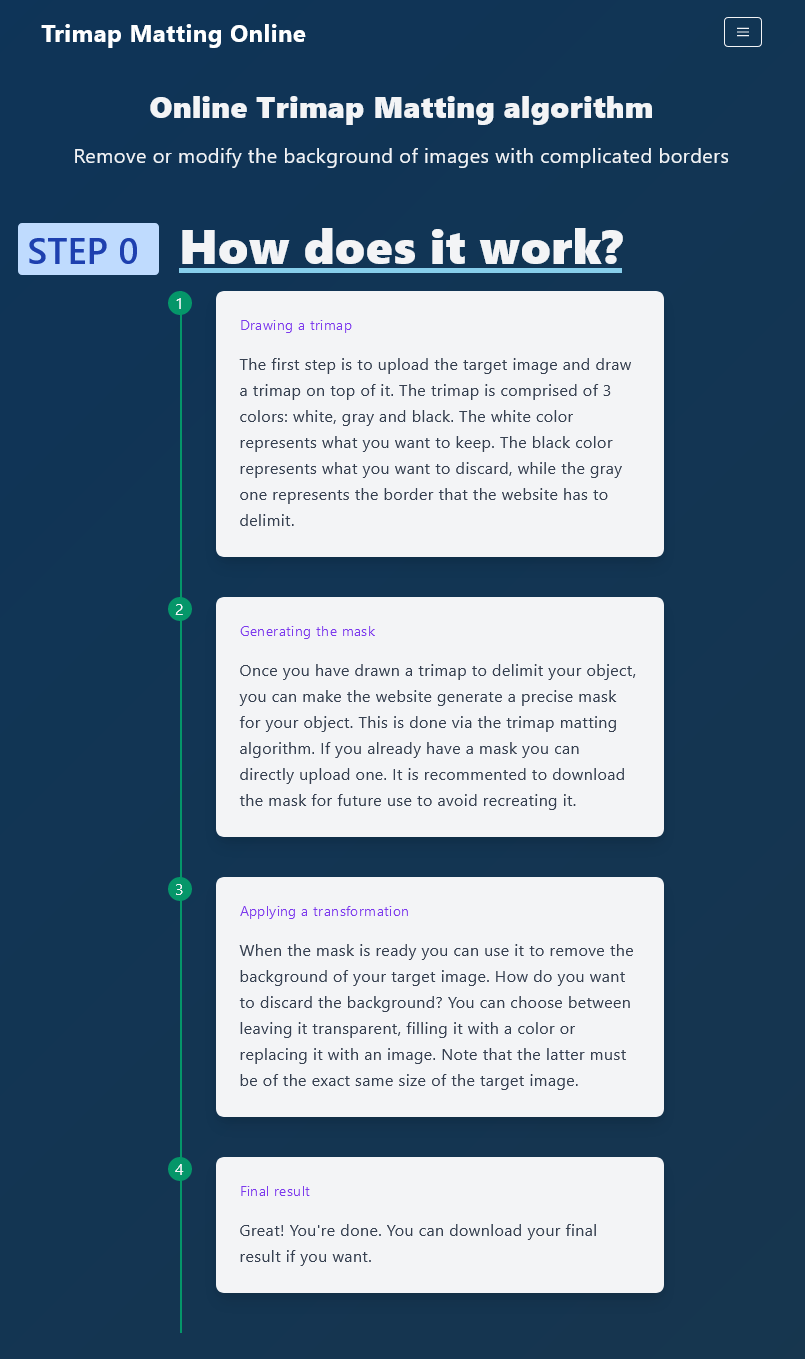
\includegraphics[width=0.7\textwidth]{website/step0.png}
    \caption{Website - Step 0}
\end{figure}

\pagebreak

The following images show the first section
of the website \textsc{STEP 1}. In this section the user is able
to upload the target image.
As shown in the first image (\ref{fig:fig1a}),
before having selected the image,
the inputs are disabled.
When an image is uploaded (\ref{fig:fig1b}),
the painting tools become available
in order to draw the trimap mask.

\begin{figure}[h]
    \centering
    \begin{minipage}[b]{0.49\textwidth}
        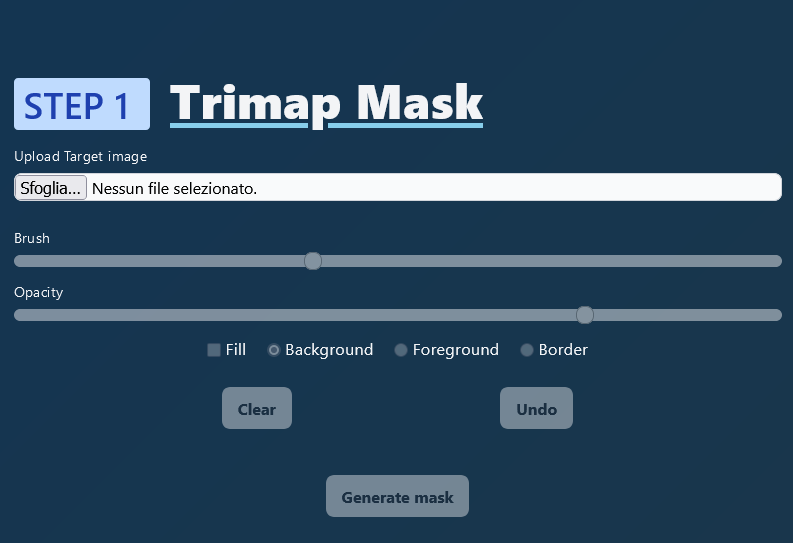
\includegraphics[width=\textwidth]{website/step1A.png}
        \label{fig:fig1a}
        \caption{Website - Step 1 A}
    \end{minipage}
    \hfill
    \begin{minipage}[b]{0.49\textwidth}
        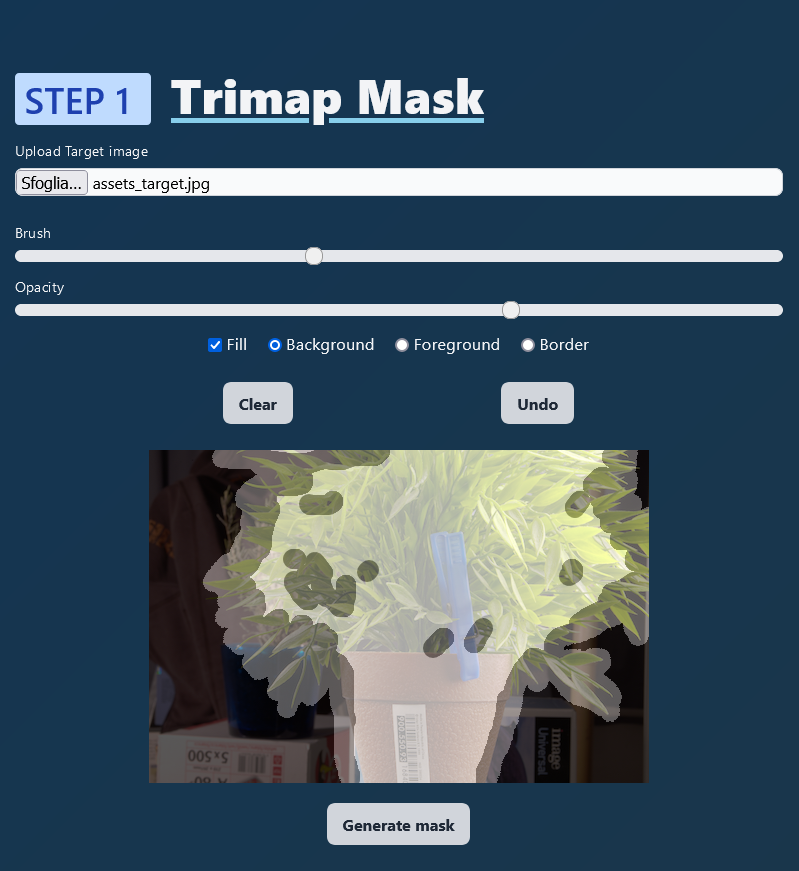
\includegraphics[width=\textwidth]{website/step1B.png}
        \label{fig:fig1b}
        \caption{Website - Step 1 B}
    \end{minipage}
\end{figure}

The following images show the second section
of the website \textsc{STEP 2}.
In this section the current alpha matte mask
is displayed. The mask can be generated by pressing
the respective button in the \textsc{STEP 1}
section. Alternatively, the user is able to
directly upload a mask from the file system
(as in \ref{fig:fig2b}).

\begin{figure}[h]
    \centering
    \begin{minipage}[b]{0.49\textwidth}
        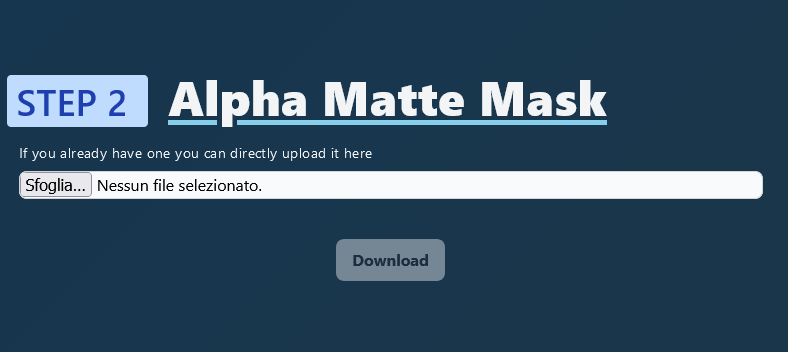
\includegraphics[width=\textwidth]{website/step2A.png}
        \label{fig:fig2a}
        \caption{Website - Step 2 A}
    \end{minipage}
    \hfill
    \begin{minipage}[b]{0.49\textwidth}
        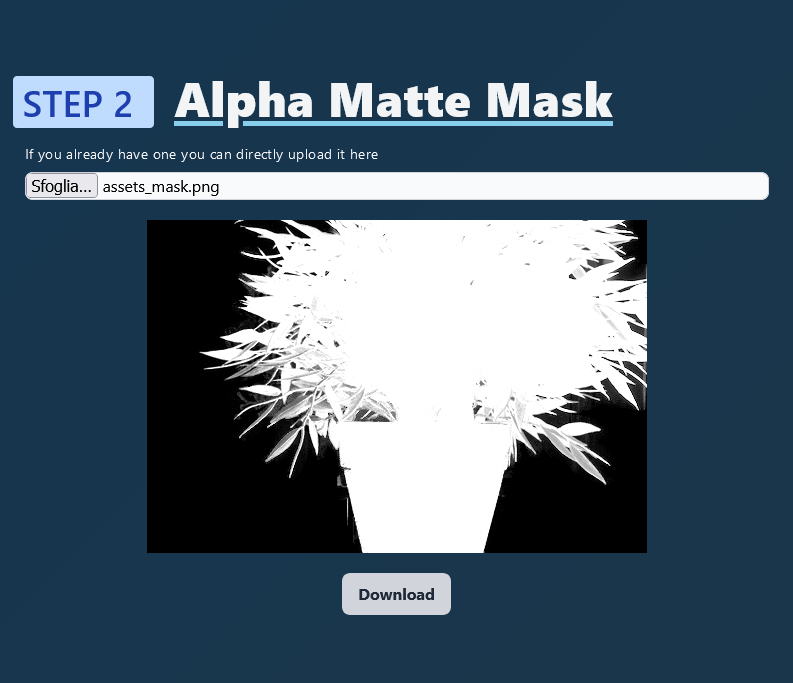
\includegraphics[width=\textwidth]{website/step2B.png}
        \label{fig:fig2b}
        \caption{Website - Step 2 B}
    \end{minipage}
\end{figure}

\pagebreak

The following images show the third section
of the website \textsc{STEP 3}.
In this section the user is able to select
a transformation to apply on the background,
which will be applied using the alpha matte mask
previosuly generated. \\
The first image (\ref{fig:fig3a}) shows the transformation
section when a mask is not yet available
in \textsc{STEP 2}. The second image (\ref{fig:fig3b})
shows the color input being used.

\begin{figure}[h]
    \centering
    \begin{minipage}[b]{0.49\textwidth}
        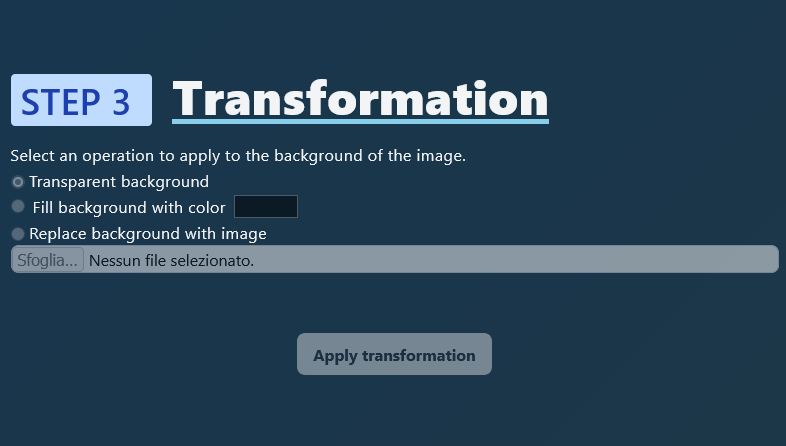
\includegraphics[width=\textwidth]{website/step3A.png}
        \label{fig:fig3a}
        \caption{Website - Step 3 A}
    \end{minipage}
    \hfill
    \begin{minipage}[b]{0.49\textwidth}
        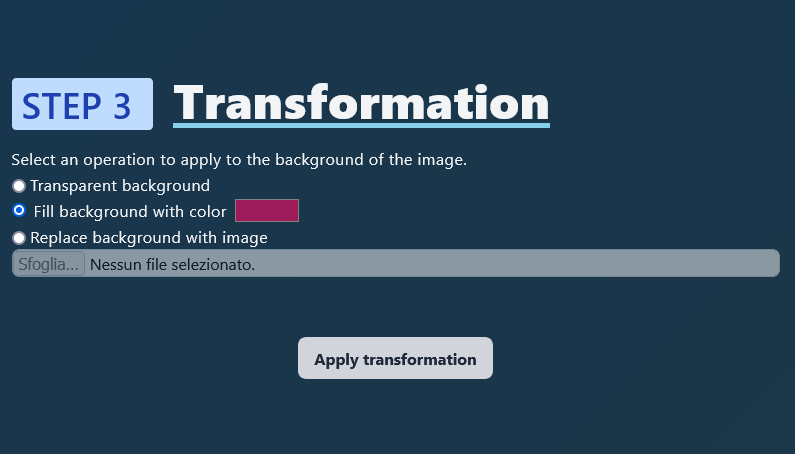
\includegraphics[width=\textwidth]{website/step3B.png}
        \label{fig:fig3b}
        \caption{Website - Step 3 B}
    \end{minipage}
\end{figure}

\begin{wrapfigure}{l}{0.5\textwidth}
    \vspace{-\intextsep}
    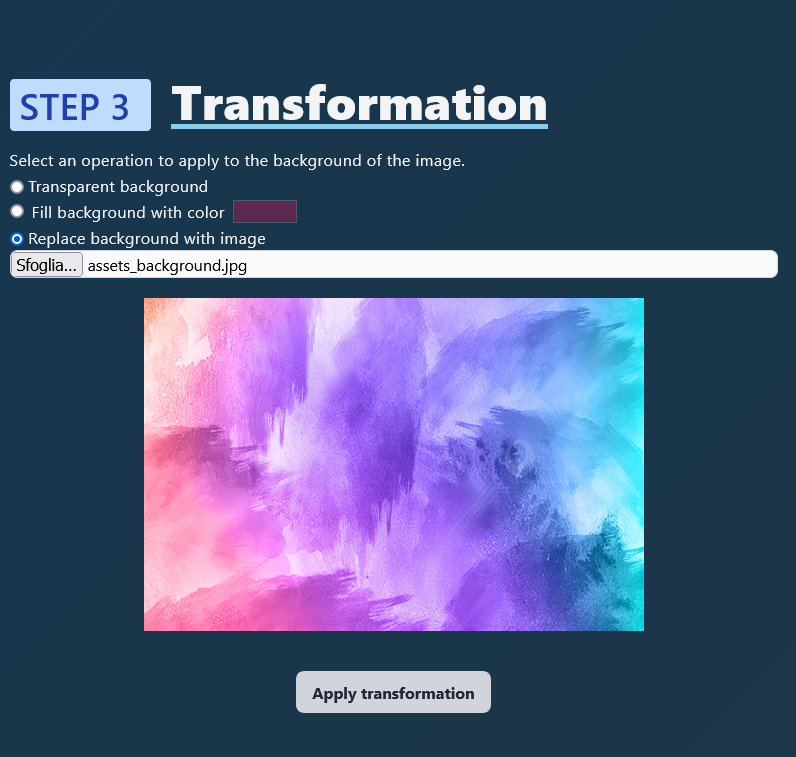
\includegraphics[width=0.5\textwidth]{website/step3C.png}
    \caption{Website - Step 3 C}
\end{wrapfigure}

This image shows the file input being used.
It is important to note that whenever one of the 3
options is selected, the other inputs are disabled.

\wrapfill

\begin{figure}[h]
    \centering
    \begin{minipage}[b]{0.49\textwidth}
        \centering
        \begin{minipage}[t]{\textwidth}
            The following images show the last section (\textsc{STEP 4}).
            This section displays the resulting image, which can be
            generated by pressing the respective button in \textsc{STEP 3}.
            \vspace{1cm}
        \end{minipage}
        
\includegraphics[width=\textwidth]{website/step4A.png}
        \caption{Website - Step 4 A}
        \label{fig:fig3a}
    \end{minipage}
    \hfill
    \begin{minipage}[b]{0.49\textwidth}
        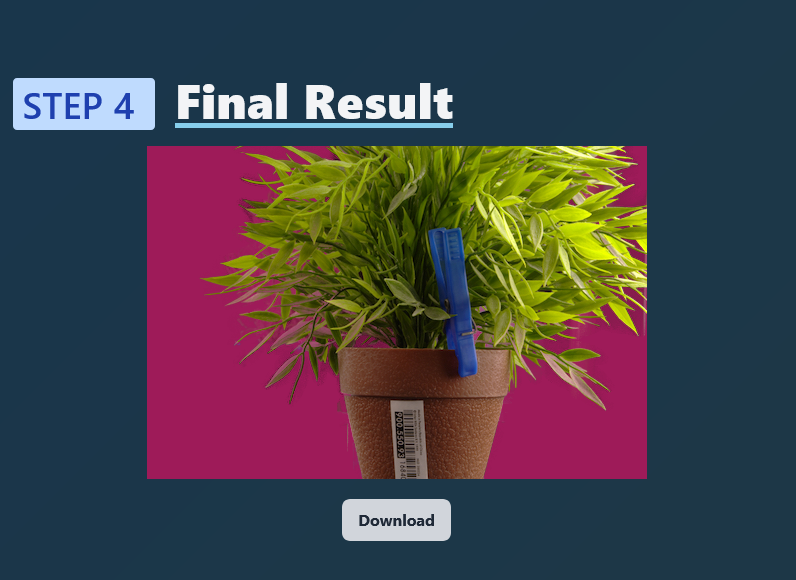
\includegraphics[width=\textwidth]{website/step4B.png}
        \caption{Website - Step 4 B}
        \label{fig:fig3b}
    \end{minipage}
\end{figure}

\pagebreak

\subsection{Dependencies}

Here's a list of all the libraries used within the project

\bgroup{}
\def\arraystretch{1.5}
\begin{center}
    \begin{tabular}{ |p{2cm}|p{4cm}|p{1.5cm}|p{2cm}| }
        \hline
        \multicolumn{4}{|c|}{\textbf{Dependency table (matting-lib)}} \\
        \hline
        \textbf{Name} & \textbf{Description} & \textbf{Version} & \textbf{Features} \\
        \hline
        opencv & Image processing & 0.78.0 & \- \\
        \hline
        image & Image processing & 0.24.5 & webp, webp-encoder \\
        \hline
    \end{tabular}
\end{center}
\egroup{}

\bgroup{}
\def\arraystretch{1.5}
\begin{center}
    \begin{tabular}{ |p{2cm}|p{4cm}|p{1.5cm}|p{2cm}| }
        \hline
        \multicolumn{4}{|c|}{\textbf{Dependency table (matting-cli)}} \\
        \hline
        \textbf{Name} & \textbf{Description} & \textbf{Version} & \textbf{Features} \\
        \hline
        clap & CLI parameters & 4.0.29 & derive \\
        \hline
        csscolorparser & CSS color parsing & 0.6.2 & \- \\
        \hline
        chrono & Timestamps & 0.4.23 & \- \\
        \hline
        matting-lib & Matting library & (local) & \- \\
        \hline
    \end{tabular}
\end{center}
\egroup{}

\bgroup{}
\def\arraystretch{1.5}
\begin{center}
    \begin{tabular}{ |p{2cm}|p{4cm}|p{1.5cm}|p{2cm}| }
        \hline
        \multicolumn{4}{|c|}{\textbf{Dependency table (matting-web)}} \\
        \hline
        \textbf{Name} & \textbf{Description} & \textbf{Version} & \textbf{Features} \\
        \hline
        warp & Web server & 0.3.3 & \- \\
        \hline
        futures & Multi threading & 0.3.25 & \- \\
        \hline
        tokio & Multi threading & 1 & full \\
        \hline
        csscolorparser & CSS color parsing & 0.6.2 & \- \\
        \hline
        clap & CLI parameters & 0.4.29 & derive \\
        \hline
        lazy\_static & Lazily evaluated statics & 1.4.0 & \- \\
        \hline
        tempfile & Temporary files & 3.4.0 & \- \\
        \hline
        matting-lib & Matting library & (local) & \- \\
        \hline
    \end{tabular}
\end{center}
\egroup{}

\pagebreak

\subsection{Logging system}

\subsubsection{Environmental variables}

The logging level and logging style can be set
by exporting the \colorbox{gray!10}{MATTING\_LOG} and \\
\colorbox{gray!10}{MATTING\_LOG\_STYLE}
environmental variables. The variables represent the log level
and the log style respectively.

The \colorbox{gray!10}{MATTING\_LOG} variable may assume the following values
\begin{itemize}
    \item \colorbox{gray!10}{error}: Designates very serious errors.
    \item \colorbox{gray!10}{warn}: Designates hazardous situations.
    \item \colorbox{gray!10}{info}: Designates useful information.
    \item \colorbox{gray!10}{debug}: Designates lower priority information.
    \item \colorbox{gray!10}{trace}: Designates very lower priority, often extremely verbose, information.
\end{itemize}
See \cite{envlogginglvl} for more information and more options.

The \colorbox{gray!10}{MATTING\_LOG\_STYLE} variable may assume the following values
\begin{itemize}
    \item \colorbox{gray!10}{auto}: Will attempt to print style characters if possible.
    \item \colorbox{gray!10}{always}: Will always print style characters.
    \item \colorbox{gray!10}{never}: Will never print style characters.
\end{itemize}
See \cite{envloggingstyle} for more information.

\subsubsection{matting-cli}

This program only uses the \colorbox{gray!10}{info}, \colorbox{gray!10}{warn}
and \colorbox{gray!10}{error} log levels.

The \texttt{--verbose} flag automatically sets \colorbox{gray!10}{MATTING\_LOG}
to \colorbox{gray!10}{\texttt{info}}. \\

\subsubsection{matting-web}

This program logs to the \colorbox{gray!10}{info},
\colorbox{gray!10}{debug},
\colorbox{gray!10}{warn}
and \colorbox{gray!10}{error} levels.

The default level is set to \colorbox{gray!10}{info}.

\pagebreak

\subsection{Flux Diagrams and Error handling}

\subsubsection{Matting CLI}

The following diagram shows the flux of the \texttt{matting-cli} executable.

\begin{figure}[h]
    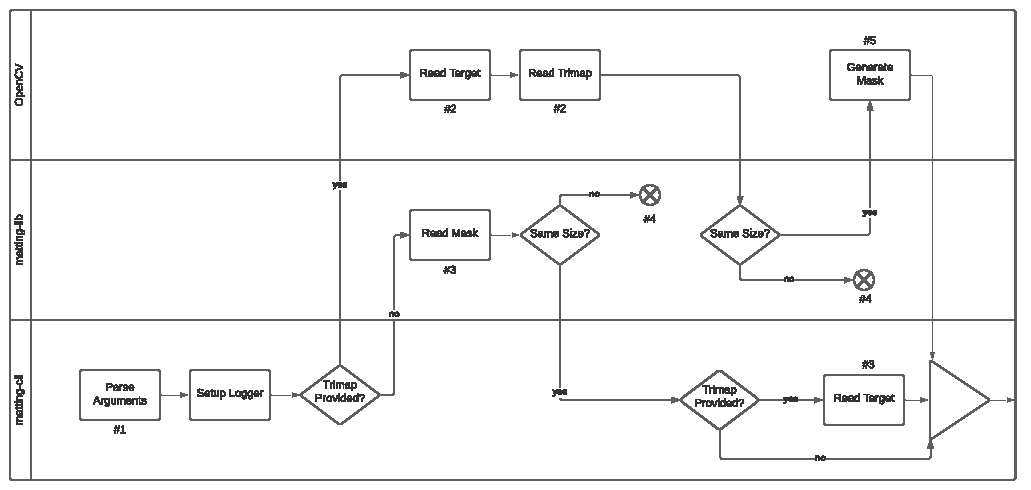
\includegraphics[width=\textwidth]{media/swimlane/swimlane1.pdf}
\end{figure}

\begin{figure}[h]
    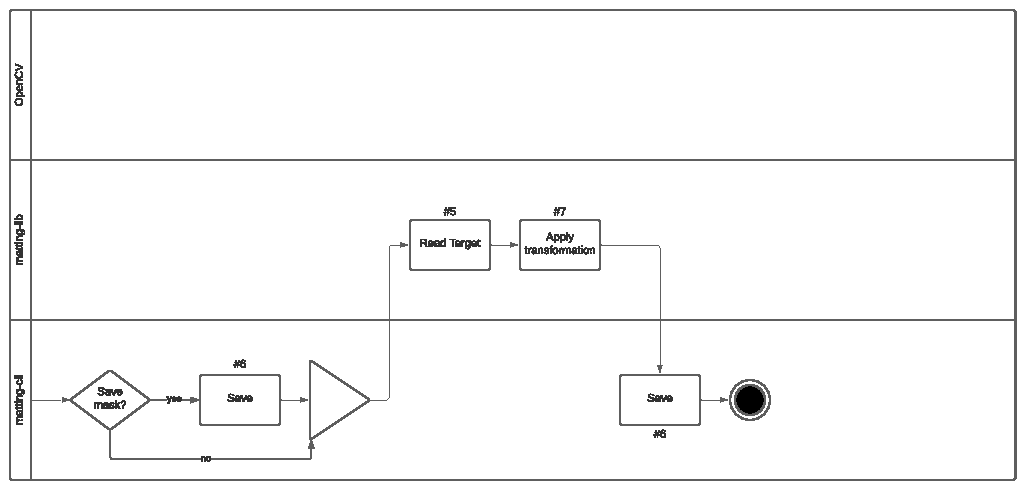
\includegraphics[width=\textwidth]{media/swimlane/swimlane2.pdf}
    \caption{CLI Swimlane}
\end{figure}

The numbered labels (\#) represent the possible errors at the given stage.

\begin{itemize}
    \item[\#1] Wrong CLI parameters or invalid combination.
    \item[\#2] (\texttt{OpenCV}) The image file is corrupt or could not be read.
        The file may not exist or the executable may not have the required
        permission.
    \item[\#3] (\texttt{matting-lib}) The image file is corrupt or could not be read.
        The file may not exist or the executable may not have the required
        permission.
    \item[\#4] The two images are not of the same size.
    \item[\#5] The mask could not be generated. \underline{This is most likely a hard core dump}.
    \item[\#6] The image could not be saved. The path may not exist or the executable
        may not have the required permission.
    \item[\#7] The color is invalid and could not be parsed.
\end{itemize}

\pagebreak

\subsubsection{Matting WEB}

Thw following diagram shows the flux of the \texttt{matting-web} executable.

\begin{figure}[h]
    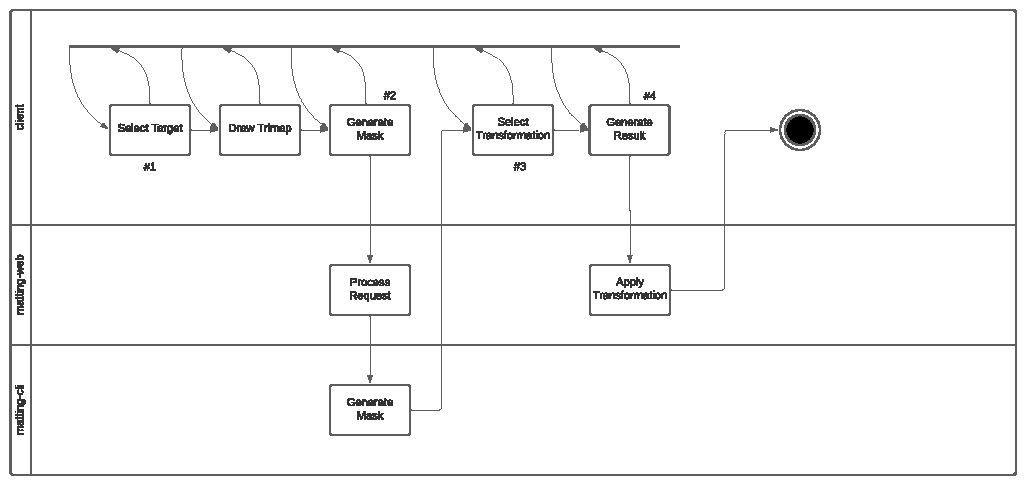
\includegraphics[width=\textwidth]{media/swimlane/swimlane3.pdf}
    \caption{WEB Swimlane}
\end{figure}

It is important to note that at every stage, the user is able
to go back to any previous stage.

The numbered labels (\#) represent the possible errors at the given stage.

\begin{itemize}
    \item[\#1] The target is not a valid image, or it is bigger than 2MiB.
    \item[\#2] The mask could not be generated.
        This is most likely a \textsc{BAD\_REQUEST}
        or \textsc{INTERNAL\_SERVER\_ERROR}.
    \item[\#3] The image size is not the same as the target.
    \item[\#4] The result could not be generated.
        This is most likely a \textsc{BAD\_REQUEST}
        or \textsc{INTERNAL\_SERVER\_ERROR}
\end{itemize}

\pagebreak

\section{Structure}

\subsection{mandate}

The \texttt{mandate} folder contains all the documents regarding
the project (documentation, abstract and diaries).

\subsection{matting-lib}

The \texttt{matting-lib} folder.

\subsection{matting-cli}

The \texttt{matting-cli} folder.

\subsection{matting-web}

The \texttt{matting-web} folder.

\subsection{assets}

The \texttt{assets} folder contains
example images and resources to use the project.
These files can be used for the testing protocol.

\pagebreak

\section{Tests}

\subsection{Testing protocol}

\subsubsection{CLI Tests}

\paragraph{Requirements:}
The following tests must be executed are satisfying the
following requirements. The resources can be found in the project source code.
Tests must be executed in order.

\begin{enumerate}
    \item The compiled executable of the matting-cli software
    must be placed in a folder specified in the \textsc{PATH}
    environmental variable (e.g. \texttt{/usr/local/bin} or \texttt{/usr/bin}).
    \item The matting-cli file must be an executable. It should be enough to run
    \lstinline{chmod +x <file>}.
    \item The user from which the tests will be executed must have permission to execute
    the program.
    \item A valid \texttt{target} image (\texttt{target.jpg}).
    \item A valid \texttt{trimap} image with the same size of the target image (\texttt{trimap.png}).
    \item A valid \texttt{background} image with the same size of the target image (\texttt{background.jpg}).
    \item The user must have the permission to read each resource used and write files
    to the specified locations.
    \item All the resources needed must be in the same directory as the one where the caller executed the commands.
    \item An image viewer with resizing capabilities along with a graphical environment.
    \item The command \texttt{file}.
\end{enumerate}

\lstdefinestyle{mattingcli} {
    basicstyle=\ttfamily,
    numbers=none,
    breaklines=true,
    backgroundcolor=\color[gray]{0.97},
    morekeywords={INFO},
    keywordstyle=\color[rgb]{0, 0.75, 0},
    morekeywords=[2]{ERROR},
    keywordstyle=[2]\color[rgb]{0.75, 0, 0},
    morekeywords=[3]{WARN},
    keywordstyle=[3]\color[rgb]{1, 0.5, 0}
}

\newcommand{\moveabit}[1]{\adjustbox{lap={\width}{-0.9cm}}{#1}}

\paragraph{Tests:}

\test{00}{Verbose output}{Req-05}{
\item
\makecell[tl]{
    Execute the following command: \\
    \moveabit{\begin{lstlisting}[style=mattingcli]^^J
        matting-cli -i target.jpg --trimap trimap.png^^J
            --save-mask mask.png -o out.png^^J
            --fill red --verbose^^J
    \end{lstlisting}}
}
}{%
\makecell[tl]{
The output written to the \textsc{stdout} must look like this: \\
\begin{lstlisting}[style=mattingcli]^^J
    [<time> INFO  matting_cli] Reading target image...^^J 
    [<time> INFO  matting_cli] Done! [<time>]^^J
    [<time> INFO  matting_cli] Reading trimap image...^^J 
    [<time> INFO  matting_cli] Done! [<time>]^^J
    [<time> INFO  matting_cli] Generating soft mask...^^J 
    [<time> INFO  matting_cli] Done! [<time>]^^J
    [<time> INFO  matting_cli] Reading target image...^^J 
    [<time> INFO  matting_cli] Done! [<time>]^^J
    [<time> INFO  matting_cli] Saving soft mask to mask.png...^^J 
    [<time> INFO  matting_cli] Done! [<time>]^^J
    [<time> INFO  matting_cli] Filling background with color...^^J 
    [<time> INFO  matting_cli] Done! [<time>]^^J
    [<time> INFO  matting_cli] Saving output to out.png...^^J 
    [<time> INFO  matting_cli] Done! [<time>]^^J
\end{lstlisting}
}
}

\test{01}{Help message}{Req-00}{
    \item 
    \makecell[tl]{
        Execute the following command: \\
        \moveabit{\begin{lstlisting}[style=mattingcli]^^J
            matting-cli -h^^J
            matting-cli --help^^J
        \end{lstlisting}}
    }
}{%
\makecell[tl]{
    The output written to the \textsc{stdout} must look like this: \\
\begin{lstlisting}[style=mattingcli]^^J
Matting CLI^^J
^^J
Usage: matting-cli [OPTIONS] --target <TARGET>^^J
                    <--mask <MASK>|--trimap <TRIMAP>>^^J
^^J
Options:^^J
    -i, --target <TARGET>        Target image^^J
        --mask <MASK>            Background mask image^^J
        --trimap <TRIMAP>        Trimap image^^J
        --save-mask <SAVE_MASK>  Save mask path^^J
    -o, --output <OUTPUT>        Output image^^J
    -f, --fill <FILL>            Fill background action^^J
    -t, --transparent            Transparent background action^^J
    -r, --replace <REPLACE>      Replace background action^^J
        --verbose                Verbose flag^^J
    -h, --help                   Print help information^^J
    -V, --version                Print version information^^J
\end{lstlisting}
}
}

\test{02}{Empty parameters}{Req-00\_0, Req-00\_1, Req-00\_2, Req-00\_3, Req-00\_4}{
    \item 
    \makecell[tl]{
        Execute the following command: \\
        \moveabit{\begin{lstlisting}[style=mattingcli]^^J
            matting-cli^^J
        \end{lstlisting}}
    }
}{%
\makecell[tl]{
    The output written to the \textsc{stdout} must look like this: \\
    \begin{lstlisting}[style=mattingcli]^^J
        error: The following required arguments were not:^^J
            provided:^^J
          --target <TARGET>^^J
          <--mask <MASK>|--trimap <TRIMAP>>^^J
          ^^J
        Usage: matting-cli --target <TARGET>^^J
            <--mask <MASK>|--trimap <TRIMAP>>^^J
            ^^J
        For more information try '--help'^^J
    \end{lstlisting}
}
}

\test{03}{Empty action}{Req-00}{
    \item 
    \makecell[tl]{
        Execute the following command: \\
        \moveabit{\begin{lstlisting}[style=mattingcli]^^J
            matting-cli --target target.jpg --trimap trimap.png^^J
        \end{lstlisting}}
    }
}{%
The output written to the \textsc{stdout} must be empty and no file must
be generated.
}

\pagebreak

\test{04}{Mask generation}{Req-00\_4}{
    \item 
    \makecell[tl]{
        Delete the previously generated mask: \\
        \moveabit{\begin{lstlisting}[style=mattingcli]^^J
            rm mask.png^^J
        \end{lstlisting}}
    }
    \item 
    \makecell[tl]{
        Execute the following command: \\
        \moveabit{\begin{lstlisting}[style=mattingcli]^^J
            matting-cli --target target.jpg --trimap^^J
                trimap.png --save-mask mask.png
        \end{lstlisting}}
    }
    \item 
    \makecell[tl]{
        List the files in the current directory: \\
        \moveabit{\begin{lstlisting}[style=mattingcli]^^J
            ls .^^J
        \end{lstlisting}}
    }
}{%
The output written to the \textsc{stdout} must be empty and a file
\texttt{mask.png} must appear in the directory.
}

\test{05}{Replace background feature}{Req-00\_5}{
    \item 
    \makecell[tl]{
        Execute the following commands: \\
        \moveabit{\begin{lstlisting}[style=mattingcli]^^J
            matting-cli -i target.jpg --trimap trimap.png^^J
                --replace background.jpg -o res1.jpg^^J
            matting-cli -i target.jpg --mask mask.png^^J
                --replace background.jpg -o res2.jpg^^J
        \end{lstlisting}}
    }
    \item Open \texttt{res1.jpg} and \texttt{res2.jpg} with an image viewer.
}{%
    Both images must present the background image behind the subject.
}

\test{06}{Fill background feature}{Req-00\_6}{
    \item 
    \makecell[tl]{
        Execute the following commands: \\
        \moveabit{\begin{lstlisting}[style=mattingcli]^^J
            matting-cli -i target.jpg --mask mask.png^^J
                --fill "red" -o res1.jpg^^J
            matting-cli -i target.jpg --mask mask.png^^J
                --fill "#FF0000" -o res2.jpg^^J
            matting-cli -i target.jpg --mask mask.png^^J
                --fill "rgb(255,0,0)" -o res3.jpg^^J
        \end{lstlisting}}
    }
    \item Open \texttt{res1.jpg}, \texttt{res2.jpg} and \texttt{res4.jpg} with an image viewer.
}{%
    Both images must present a red colored background behind the subject.
}

\test{07}{Transparent feature}{Req-00\_7}{
    \item 
    \makecell[tl]{
        Execute the following commands: \\
        \moveabit{\begin{lstlisting}[style=mattingcli]^^J
            matting-cli -i target.jpg --trimap trimap.png^^J
                --transparent -o res1.png^^J
            matting-cli -i target.jpg --mask mask.png^^J
                --transparent -o res2.png^^J
        \end{lstlisting}}
    }
    \item Open \texttt{res1.png} and \texttt{res2.png} with an image viewer.
}{%
    Both images must present a transparent background behind the subject.
}

\test{08}{Output with format}{Req-01}{
    \item 
    \makecell[tl]{
        Execute the following commands: \\
        \moveabit{\begin{lstlisting}[style=mattingcli]^^J
            matting-cli -i target.jpg --mask mask.png^^J
                --fill "red" -o format.webp^^J
            matting-cli -i target.jpg --mask mask.png^^J
                --fill "red" -o format.jpg^^J
            matting-cli -i target.jpg --mask mask.png^^J
                --fill "red" -o format.png^^J
        \end{lstlisting}}
    }
    \item 
    \makecell[tl]{
        Print information about each of the resulting images: \\
        \moveabit{\begin{lstlisting}[style=mattingcli]^^J
            file format.webp^^J
            file format.jpg^^J
            file format.png^^J
        \end{lstlisting}}
    }
}{%
\makecell[tl]{
    Each information line must specificy the respective image format. \\
    (e.g. \texttt{.jpg} \(\rightarrow\) \textsc{JPG})
}
}

\test{09}{Transparency and JPG format}{None}{
    \item 
    \makecell[tl]{
        Execute the following command: \\
        \moveabit{\begin{lstlisting}[style=mattingcli]^^J
            matting-cli -i target.jpg --mask mask.png^^J
            --transparent -o res.jpg^^J
        \end{lstlisting}}
    }
    \item Open \texttt{res.jpg} with an image viewer.
}{%
\makecell[tl]{
    A message to the \textsc{STDOUT} must warn about the usage of the JPG format \\
    with transparency. The image must have a black background behind the\\
    subject. \\
    \begin{lstlisting}[style=mattingcli]^^J
    [<date> WARN  matting_cli] The image has an alpha channel but the format is not PNG.^^J
    [<date> WARN  matting_cli] It is advised to change the output format to ".png"^^J
    \end{lstlisting}
}
}

\test{10}{Mask default name}{Req-04}{
    \item 
    \makecell[tl]{
        Execute the following command: \\
        \moveabit{\begin{lstlisting}[style=mattingcli]^^J
            matting-cli -i target.jpg --trimap trimap.png^^J
            --save-mask^^J
        \end{lstlisting}}
    }
    \item List the files in the directory
}{%
The mask must have been saved in the current directory with the name \texttt{mask\_[timestamp].png}.
}

\test{11}{Output default name}{Req-04}{
    \item 
    \makecell[tl]{
        Execute the following command: \\
        \moveabit{\begin{lstlisting}[style=mattingcli]^^J
            matting-cli -i target.jpg --mask mask.png^^J
            --transparent^^J
        \end{lstlisting}}
    }
    \item \makecell[tl]{
        List the files in the current directory: \\
        \moveabit{\begin{lstlisting}[style=mattingcli]^^J
            ls .^^J
        \end{lstlisting}}
    }
}{%
The mask must have been saved in the current directory with the name \texttt{target\_[timestamp].png}.
}

\test{12}{Wrong size images}{Req-02}{
    \item Copy \texttt{trimap.png}, \texttt{mask.png} and \texttt{background.jpg} to
        \texttt{trimap2.png}, \texttt{mask2.png} and \texttt{background2.jpg} respectively.
    \item Open \texttt{trimap2.png}, \texttt{mask2.png} and \texttt{background2.jpg}
        and resize them to a smaller dimension.
    \item Save the files.
    \item 
    \makecell[tl]{
        Execute the following commands: \\
        \moveabit{\begin{lstlisting}[style=mattingcli]^^J
            matting-cli -i target.jpg --mask mask2.png^^J
            matting-cli -i target.jpg --trimap trimap2.png^^J
            matting-cli -i target.jpg --mask mask.png^^J
                --replace background2.jpg^^J
        \end{lstlisting}}
    }
}{%
\makecell[tl]{
    Each of the matting commands must print en error indicating that the sizes \\
    of the images are not the same. \\
    \begin{lstlisting}[style=mattingcli]^^J
        [<time> ERROR matting_cli] An error occured: The mask and target image must be of the same size.^^J
        [<time> ERROR matting_cli] An error occured: The trimap and target image must be of the same size.^^J
        [<time> ERROR matting_cli] An error occured: The replacement and target image must be of the same size.^^J
    \end{lstlisting}
}
}

\pagebreak

\subsubsection{Website Tests}

\paragraph{Requirements:}
The following tests must be executed are satisfying the
following requirements. The resources can be found in the project source code.
Tests must be executed in order.

\begin{enumerate}
    \item The compiled executable of the matting-cli software
    must be placed in a folder specified in the \textsc{PATH}
    environmental variable (e.g. \texttt{/usr/local/bin} or \texttt{/usr/bin}).
    \item The matting-cli file must be an executable. It should be enough to run
    \lstinline{chmod +x <file>}.
    \item A browser.
    \item The user from which the tests will be executed must have permission to execute
    the program.
    \item A valid \texttt{target} image (\texttt{target.jpg}).
    \item A valid \texttt{trimap} image with the same size of the target image (\texttt{trimap.png}).
    \item A valid \texttt{background} image with the same size of the target image (\texttt{background.jpg}).
    \item A running server instance of the web application.
    \item The server must have the permission to read each resource used and write files
    to the specified locations.
    \item The server must have read and write permissions to \texttt{/tmp}.
\end{enumerate}

\paragraph{Tests:}

\test{13}{Trimap mask generation}{Req-03}{
    \item Upload the target image to the website
    \item Draw the trimap with the given tools
    \item Press the generate mask button
}{%
    A loading animation must appear on the website.
    After some time the corresponding alpha matte mask must appear, replacing the loading animation.
}

\test{14}{Save mask feature}{Req-03}{
    \item Press the download button under the generated mask image
    \item Open the image from the file system with a viewer
}{%
    The image must be saved and contain the correct image.
}

\test{15}{Transparency feature}{Req-03}{
    \item Select the transparent transformation option
    \item Click the apply transformation button 
}{%
A loading animation must appear on the website.
After some time the corresponding alpha matte mask must appear, replacing the loading animation.
The result must be the target image with a transparent background.
}

\test{16}{Fill background feature}{Req-03}{
    \item Select the fill background transformation option
    \item Select a color with the color input
    \item Click the apply transformation button 
}{%
A loading animation must appear on the website.
After some time the corresponding alpha matte mask must appear, replacing the loading animation.
The result must be the target image with the selected color as a background.
}

\test{17}{Replace background feature}{Req-03}{
    \item Select the transparent transformation option
    \item Select the background image with the file input
    \item Click the apply transformation button 
}{%
A loading animation must appear on the website.
After some time the corresponding alpha matte mask must appear, replacing the loading animation.
The result must be the target image with the selected image as a background.
}

\test{18}{Save result feature}{Req-03}{
    \item Press the download button under the generated image
    \item Open the image from the file system with a viewer
}{%
    The image must be saved and contain the correct image.
}

\test{19}{Wrong size replacement}{Req-03}{
    \item Select the replacement background option as a transformation
    \item Upload the \texttt{background2.jpg} image
}{%
    An alert message must appear saying that the background
    must be of the same size as the target image.
}

\test{20}{Core dump}{Req-03}{
    \item Draw the trimap such that it all black
    \item Press the generate mask button
}{%
    The server must not crash and keep running
}

\test{21}{Image size cap}{Req-03}{
    \item Upload an image with size bigger than 2MiB as the target image
}{%
    An alert must appear saying that the image size cannot exceed 2MiB of size.
}

\pagebreak

\test{22}{Empty parameters}{Req-03}{
    \item 
    \makecell[tl]{
        Execute the following command: \\
        \moveabit{\begin{lstlisting}[style=mattingcli]^^J
            matting-web^^J
        \end{lstlisting}}
    }
}{%
\makecell[tl]{
    The output written to the \textsc{stdout} must look like this: \\
    \begin{lstlisting}[style=mattingcli]^^J
        error: the following required arguments were not provided:^^J
        --www <WWW>^^J
        ^^J
      Usage: matting-web --www <WWW>^^J
      ^^J
      For more information, try '--help'.^^J
    \end{lstlisting}
}
}

\test{23}{Logging}{Req-05}{
    \item 
    \makecell[tl]{
        Execute the following command: \\
        \moveabit{\begin{lstlisting}[style=mattingcli]^^J
            matting-web -w <path/to/www>^^J
        \end{lstlisting}}
    }
}{%
\makecell[tl]{
The output must look like this and keep logging. \\
\begin{lstlisting}[style=mattingcli]^^J
    [<time> INFO  matting_web::handler] Server starting^^J
    [<time> INFO  warp::server] Server::run; addr=0.0.0.0:8080^^J
    [<time> INFO  warp::server] listening on http://0.0.0.0:8080^^J
\end{lstlisting}
}
}

\pagebreak

\subsection{Test results}

\definecolor{darkgreen}{rgb}{0, 0.6, 0.2}
\bgroup{}
\def\arraystretch{1.25}
\begin{center}
    \begin{tabular}{ |l|l|l| }
        \hline
        \textbf{ID} & \textbf{Result} & \textbf{Note} \\
        \hline
        \textbf{Test-00} & \color{darkgreen} Passed & The output looks like the given one. \\
        \hline
        \textbf{Test-01} & \color{darkgreen} Passed & The output looks like the given one. \\
        \hline
        \textbf{Test-02} & \color{darkgreen} Passed & The output looks like the given one. \\
        \hline
        \textbf{Test-03} & \color{darkgreen} Passed & Nothing was done. \\
        \hline
        \textbf{Test-04} & \color{darkgreen} Passed & Empty \textsc{stdout} and correct mask generated. \\
        \hline
        \textbf{Test-05} & \color{darkgreen} Passed & The background is correct. \\
        \hline
        \textbf{Test-06} & \color{darkgreen} Passed & The background is red. \\
        \hline
        \textbf{Test-07} & \color{darkgreen} Passed & The background is transparent. \\
        \hline
        \textbf{Test-08} & \color{darkgreen} Passed & Every format is correct. \\
        \hline
        \textbf{Test-09} & \color{darkgreen} Passed & A warning message is given. \\
        \hline
        \textbf{Test-10} & \color{darkgreen} Passed & The mask is saved with the correct name. \\
        \hline
        \textbf{Test-11} & \color{darkgreen} Passed & The mask is saved with the correct name. \\
        \hline
        \textbf{Test-12} & \color{darkgreen} Passed & Error messages are given. \\
        \hline
        \textbf{Test-13} & \color{darkgreen} Passed & The mask is correctly generated. \\
        \hline
        \textbf{Test-14} & \color{darkgreen} Passed & The image is correctly saved. \\
        \hline
        \textbf{Test-15} & \color{darkgreen} Passed & The result has a transparent background. \\
        \hline
        \textbf{Test-16} & \color{darkgreen} Passed & The result has a colored background. \\
        \hline
        \textbf{Test-17} & \color{darkgreen} Passed & The result has an image as a background. \\
        \hline
        \textbf{Test-18} & \color{darkgreen} Passed & The image is correctly saved. \\
        \hline
        \textbf{Test-19} & \color{darkgreen} Passed & An alert message is displayed. \\
        \hline
        \textbf{Test-20} & \color{darkgreen} Passed & The server does not crash. \\
        \hline
        \textbf{Test-21} & \color{darkgreen} Passed & An alert message is displayed. \\
        \hline
        \textbf{Test-22} & \color{darkgreen} Passed & The output looks like the given one. \\
        \hline
        \textbf{Test-23} & \color{darkgreen} Passed & The output looks like the given one. \\
        \hline
    \end{tabular}
\end{center}
\egroup{}

\pagebreak

\section{Conclusion}

\subsection{Future development}

There are lots of features that could be added to the application
and improvements that could be made.

\begin{enumerate}
    \item \textbf{GPU Acceleration}: The code remove, replace or fill the background
    of an image given its mask is executed pixel-by-pixel by the CPU.
    It would be incredibly faster if it could use the GPU instead, by using
    a library like \textit{Vulkan}. The implementation would require
    writing a simple compute shader which reads the mask and the original image
    from a buffer.
    \item \textbf{Better website}: The website design could be improved. It is not
    fully responsive and it certainly could have a better design overall.
    \item \textbf{Trimap upload}: It could be useful if the user was able to
    directly upload a trimap for a given image, rather than having to always draw it.
    \item \textbf{Automatic cropping}: When a user upload an image replacement for the background.
    It would be useful if it could be cropped to the correct size directly within the website.
    \item \textbf{Website format handling}: Unlike the CLI version, the web application does
    not handle different formats. Everything is converted into a PNG and saved as one.
    The user has to manually convert the resulting image into another format.
    \item \textbf{Optimized undo}: The undo feature gets slow as more
    flood fills are made.
\end{enumerate}

\subsection{Personal conclusions}

I really enjoyed this project for its semplicity and usefulness.

\pagebreak

\listoffigures

\pagebreak

\nocite{*} % cite all entries

\printbibliography

\pagebreak

\printnoidxglossary

\end{document}